%\begin{savequote}[8cm]
%\textlatin{Neque porro quisquam est qui dolorem ipsum quia dolor sit amet, consectetur, adipisci velit...}

%There is no one who loves pain itself, who seeks after it and wants to have it, simply because it is pain...
%  \qauthor{--- Cicero's \textit{de Finibus Bonorum et Malorum}}
%\end{savequote}

\chapter{BLDA prioritizes accessible regulatory regions in MLL-AF4 driven leukemia} \label{ch4}

\minitoc



% remember to put the process of making the MLL specific blacklist on the 



% motifs
% n=5   
% topic 3 
    % NFYC diffexp in apl https://genomebiology.biomedcentral.com/articles/10.1186/gb-2008-9-2-r38
%   % AHR crucial for leukemia stem cell maintenance https://cancerres.aacrjournals.org/content/79/22/5799
%   % CUX1 involved in myeloid leukemias https://ashpublications.org/blood/article/121/6/975/31447/CUX1-is-a-haploinsufficient-tumor-suppressor-gene 
%   % ZFX https://pubmed.ncbi.nlm.nih.gov/24485662/
% 
% NEUROG2 is also enriched, the only one not associated with leukemia of some sort. 
% shown to create distinct chromatin accessibility landscapes in very distinct neuron subpopulations https://www.ncbi.nlm.nih.gov/pmc/articles/PMC6556771/

% topic 1
%   CREB1 is a "suspected leukemia ocoprotein" https://pubmed.ncbi.nlm.nih.gov/23000483/
%           also CREM found
%      bind cAMP response elements (cAMP-response element)
%       important for normal hematopoiesis https://www.ncbi.nlm.nih.gov/pmc/articles/PMC2214769/
%        Overly expressed both in the boen marrow and blast cells of acute leukemia patients
%   MAX is differentially expressed in human myloid leukemias https://pubmed.ncbi.nlm.nih.gov/7500645/

%  topic 2
%   LIN54 is a cell cycle gene which makes sense given its enrichement in normal pre b cells https://www.nature.com/articles/ncomms12301


% 30% of cells in the RS4;11 paper resembled myeloid cells cytochemically. 
%       they were from a relapsed patient https://pubmed.ncbi.nlm.nih.gov/3917311/#:~:text=A%20cell%20line%2C%20designated%20RS4,7.
%       morphologically, they were all lymphoid in appearance

% SEM cells also from a 5 year old in relapse 
%   Lymphoid cells but also had some myeloid antigens like CD13, CD15, and CD33 https://onlinelibrary.wiley.com/doi/pdf/10.1111/j.1365-2141.1994.tb04726.x?casa_token=wybBr2k2O-QAAAAA:M5peYc4iAuyTaA7HhoEKQd-IgOQ15B6dm9_EPi-Od1UZpl5aKSTUxYT2B8IXkgYkPlaq5QfJpmLDJqk


\section{Introduction} \label{ch5:intro}

\section{Methods} \label{ch5:methods}

\section{Results} \label{ch5:results}

\subsection{MLL-AF4 in the context of other blood cells}

\subsubsection{Identifying MLL-AF4 specific accessibility patterns}

Within the context of the entire ENCODE dataset, the MLL-AF4 cells were indistinguishable from the closely related B cell precursors. In order to identify differences between them, the model would need a very large number of topics, sufficient to explain all of the detailed similarities between the diverse set of celltypes represented in the dataset. This is computationally difficult, and risks over-parameterizing the data. A reasonable alternative is a detailed examination of these cells in isolation, and a comparison to the results generated in the larger model. In this section, I create a topic model with just the cells of interest and attempt to differentiate them based on patterns in accessible chromatin using BLDA.

We once again use lanceotron to call peaks from the different cell lines. The number of called peaks differed significantly between experiments (\Cref{fig:mll_peak_calls}A). The most peaks were found in SEM and RS4;11, and the fewest were identified in Patient 3. In the latter case, it is suspected that the known low quality of this sample affected the sequencing, causing an anomalously low number of peaks to be identified. To confirm this, we use megadepth to calculate the average read coverage under identified peak regions \cite{Wilks2021} (\Cref{table:mll_cov}). Unexpectedly, patient 2 showed comparable read coverage to the other samples, while Patient 3 had anomalously low read coverage under the identified peak regions. An unremarkable number of peaks were identified in patient 3. The remainder of the samples have high coverage values sufficient to identify high quality peaks. These results encourage caution when interpreting any topic modelling on both patients 2 and 3.  


% Please add the following required packages to your document preamble:
% \usepackage{booktabs}
\begin{table}[]
    \centering
    \begin{tabular}{@{}llr@{}}
    \toprule
    Sample Identifier & Sample Alias & Coverage \\ \midrule
    Patient 11911     & Patient 1    & 884.3                        \\
    Patient 21940     & Patient 2    & 801.0                        \\
    Patient 26754     & Patient 3    & 478.8                        \\
    Patient 27800     & Patient 4    & 809.2                        \\
    PPB\_95R          & PPB 1        & 1361.5                       \\
    PPB\_75           & PPB 2        & 1610.6                       \\
    PPB\_23           & PPB 3        & 1295.9                       \\
    PB\_95R           & PB 1         & 1776.3                       \\
    PB\_75            & PB 2         & 1242.6                       \\
    PB\_23            & PB 3         & 1405.6                       \\
    RS411             & RS411        & 701.8                        \\
    SEM               & SEM          & 725.3                        \\ \bottomrule
    \end{tabular}
    \caption{Average coverage in peak regions for each sample calculated with megadepth.}
    \label{table:mll_cov}
\end{table}

Here we are comparing two methods, BLDA and cisTopic. cisTopic uses as its input a binary accessibility matrix, while BLDA uses a quantitative measure of relative coverage. To understand the structure of input to cisTopic, we plot the number of shared peak regions between the samples (\Cref{fig:mll_peak_calls}). Patient samples are overall dissimilar from \gls{bcp} and the cell lines. Consistent with the number of available peak calls, patient 2 shares the fewest peaks with the other samples. This is explainable by the low numbers of peaks in patient 2 in general. Between the two cell lines, SEM shares significantly more peaks with the \gls{bcp} than RS4;11 does (paired $T$-test P=2.56e-4). Surprisingly, there is no evidence for increased sharing within either PPB or PB cells ($T$-test P=0.595). These patterns of sharing will be important when interpreting the raw differential peak topic modelling versus the qualitative BLDA results.

\subsubsection{An MLL-AF4 specific accessibility blacklist}

Cell lines maintained in culture accumulate genetic differences over time, some of which may be advantageous to their survival in culture. \cite{Liu2019}\textcite{Ben-David2018} studied the genetic baseline for the same cell line matured in different laboratories and identified copy number gains and loses, insertions and deletions (indels) and chromosomal translocations affecting large portions of the genome in cell lines which were not shared across laboratories. Latent structural differences between the cell lines in question and the reference genome pose a particularly concerning confounding factor to the interpretation of topic modelling; differences in mappability between regions reflected in abnormal peaks unrelated to biological differences between cell types would contaminate pathway and motif enrichment analyses. To ameliorate concerns associated with structural diversity in the RS4;11 and SEM cell lines within our laboratory environment, we construct a list of regions whose enrichment is solely due to technical issues such as biases in mappability.

% These numbers are still fine
To do so, we assemble collection of input tracks to ChIP-seq analysis conducted on the RS4;11 and SEM cells in question. Briefly, these input tracks represent sonicated DNA that has not been pulled down. As such, it represents a proxy for the genomic background of sequencing noise, and regions where pileups occur are theoretically devoid of any biological meaning, and therefore represent technical artifacts. Peak calling is performed using Macs2 with an extremely stringent Q value cutoff, 0.00001, in order to preserve as much of the accessible genome as possible while eliminating the most obvious signals of technical artifacts. The resulting merged blacklist contains 21068 short regions (average $\pm$ standard deviation length = 483 $\pm$ 342 base pairs) covering 10.1 megabases of sequence in total. This blacklist is combined with the blacklist of accessible regions from the ENCODE project (CITE). The combined list covers 21.3 megabases of sequence, which we exclude from all subsequent analyses.

\begin{figure}
    \centering
    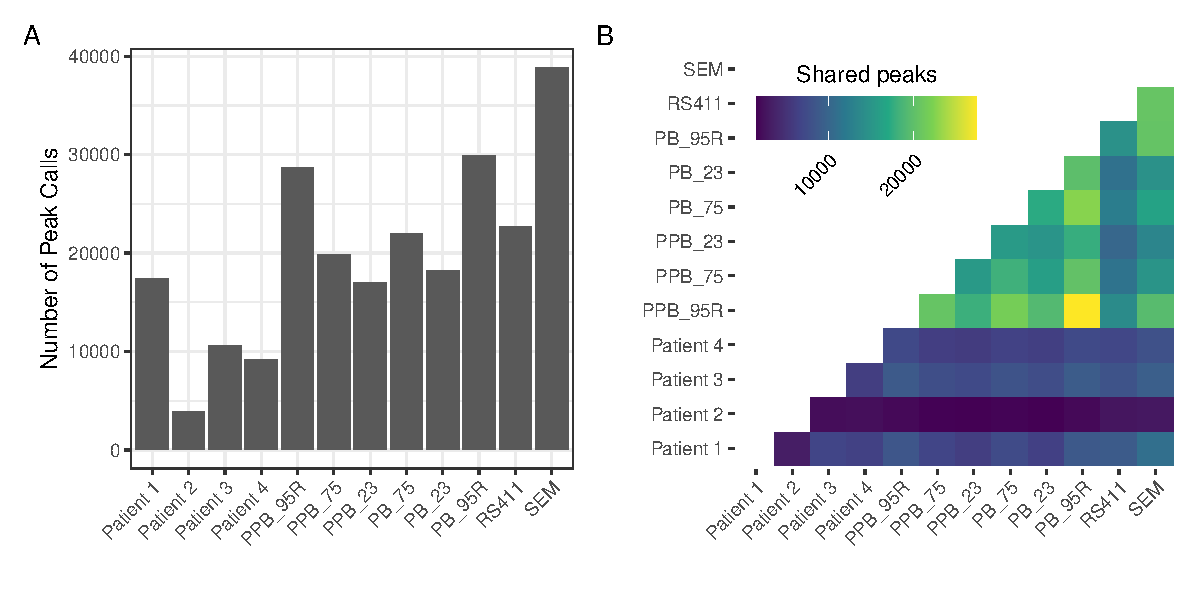
\includegraphics[width=\textwidth]{plot/ch5/mll_redo_shared_peaks.pdf}
    \caption{Peak calling of MLL-AF4 and B Cell Precursor cells with LanceOTron. A. Raw number of peak calls per cell. B. Number of shared peak calls between pairs of cells.}
    \label{fig:mll_peak_calls}
\end{figure}

% These numbers are out-dated. Not top priority to redo this. It doesn't really matter and would be similar in any case.
To justify this approach and the necessity of removing blacklisted regions, we perform the entire LDA analysis using unfiltered data, inferred topic loadings not shown. We performed region selection using the top 100, 250, and 500 regions in each topic for $k=5, \ldots, 10$ topics and found the strict overlap between the identified regions and those identified as being a part of either the ENCODE blacklist, or the ENCODE blacklist plus our custom MLL-AF4 blacklist (\Cref{fig:mll_bl_olap}). Overall, between 20.1\% and 48.8\% of the selected regions for different values of $k$ and the thresholds overlapped with ENCODE blacklisted regions. Between 51.1\% and 74.5\% of the same additionally overlapped with the custom made MLL-AF4 blacklist. 
This is compared to an overall overlap of 5998 ENCODE blacklist regions from 249903 total regions for the analysis (2.4\%) and 83434 total regions overlapping with the MLL-AF4 blacklist (33.3\%). \todo{These are from the bigwig\_merged.bed which has duplicates of the regions, so the numbers here are inflated, total is only around 63k so the others should be correspondingly less}
The blacklisted regions were therefore over-represented in the keyword regions, as expected. This analysis reaffirms the need to filter blacklisted regions.

\begin{figure}
    \centering
    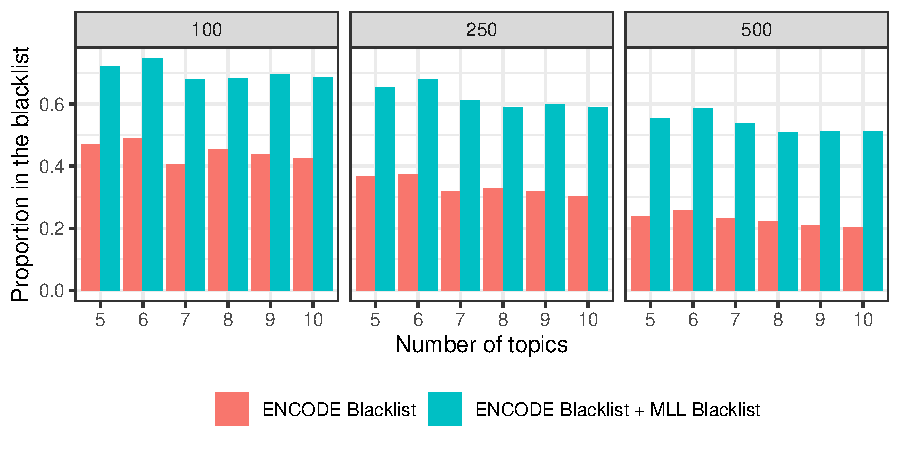
\includegraphics[width=\textwidth]{plot/ch5/mll_bl_olap.pdf}
    \caption{In an unfiltered LDA analysis of MLL-AF4 and B cell precursor cells, blacklisted regions made up the majority of identified keyword regions. Plotted is the total number of regions overlapping either of the two blacklists for a given $k$ value and the top number of regions indicated in the facet label. }
    \label{fig:mll_bl_olap}
\end{figure}

\subsubsection{Differential Accessibility between B cell Precursors and MLL-AF4 cells} \label{ch5:mll_diffacc}

After filtering out regions which overlapped with either the ENCODE or MLL-AF4 blacklist, we construct a count matrix using RPKM normalized read counts to test for baseline differential accessibility. We initially test for differential accessibility between the MLL-AF4 samples (Patients 1 through 4, RS411, and SEM) and the \gls{bcp} (PPB 1-3, PB 1-3). edgeR is used to identify differentially accessible regions between the two groups based on read counts. Overall, 27970 of the total 64162 regions were differentially accessible at a Q value threshold of 0.05. This is, however, too large a number to reasonably analyse in depth, so we select the top 100, 250, and 500 differentially accessible regions, all of which achieved statistical significance. We use GREAT to conduct an association analysis between these regions and pre-defined biological pathways. The background against which enrichment should be calculated is set to be union of all peak regions from the samples, in order to mitigate the inherent bias of analyzing accessible regions in the genome. All three subsets were enriched for Gene Ontology pathways, including peptidyl-threonine phosphorylation (4.97 fold enrichment, Q = $2.0e-7$), peptidyl-threonine modification (4.31 fold enrichment, Q = 2.4e-6), peptidyl-serine phosphorylation (2.59 fold enrichment, Q = 1.85e-2) and nucleic acid phosphodiester bond hydrolysis (2.62 fold enrichment, Q = 1.67e-2). The regions were also enriched for proximity to several genes, all of which with a corrected FDR Q value lower than 0.05 are shown in \Cref{tab:table:mll_edger_genes}.  Some of these genes are of immediate interest, including RHOU which promotes adhesion of T-cell \gls{all} cells via $\beta_1$ integrin, potentially implicating the protein in known impaired transendothelial migration potential of various kinds of leukemia cells \cite{Trinidad2009, Infante2013}. It is difficult to comprehensively survey this list of genes because their relationship with the identified regions is purely statistical. We have no mechanistic reason to believe that they are truly associated with disease. 

% Top 100, 250, and 500 motif enrichment maybe? Where are the regions?
\begin{table}

    \caption{\label{tab:table:mll_edger_genes}Enriched genic regions from the top 500 regions differentially accessible betwen MLL-AF4 cells and BCP using edgeR.}
    \centering
    \begin{tabular}[t]{llr}
    \toprule
    Gene & FDR Q Value & Fold Enrichment\\
    \midrule
    REXO1L1P & 1.41e-33 & 62.85\\ %p
    PSKH2 & 3.70e-30 & 67.37\\ 
    FOXD4L5 & 1.29e-15 & 61.60\\
    CBWD6 & 2.08e-10 & 52.50\\
    FRG2B & 4.75e-09 & 74.86\\
    \addlinespace
    RNF187 & 4.61e-09 & 51.33\\
    RHOU & 8.52e-07 & 28.52\\
    FAM27E3 & 8.54e-07 & 39.06\\
    DUX4L3 & 7.51e-06 & 128.32\\
    FOXD4L4 & 3.36e-05 & 102.66\\
    \addlinespace
    FOXD4L2 & 7.39e-05 & 29.61\\
    SERF1A & 1.94e-04 & 73.33\\
    SMN2 & 3.55e-04 & 64.16\\
    DUX4L4 & 6.23e-04 & 128.32\\
    SPATA31A5 & 2.12e-03 & 42.77\\
    \addlinespace
    ANKRD30B & 1.19e-02 & 28.52\\
    \bottomrule
    \end{tabular}
\end{table}

\subsection{Topic modelling for MLL-AF4 cells}

The focus of this chapter is an in depth investigation into using topic modelling for MLL-AF4 cells. Here, we aim to discover novel pathways that differentiate MLL-AF4 cells and normal \gls{bcp}. We do this by firstly identifying a reasonable number of topics to analyse further based on patterns in topic sharing that we observe. Secondly, we select a specific number of topics and replicate the analysis a number of times. We do this to assess the contribution of stochasticity to the inference procedure. Gibbs sampling is an approach based on Monte Carlo sampling, and as such the quality of the sampled posterior distribution can depend on the starting conditions and the convergence of the algorithm. By explicitly taking into account several repetitions of the inference algorithm we attempt to minimize the effect of chance on identified key regions. 

Similar to the above cases, peak calling is performed with LanceOTron and a score threshold of 0.5, as recommended. We construct a count matrix using the normalized read counts under each peak with BLDA as well as a one-hot encoded matrix for comparison.  Hyper-parameters alpha and beta are set for a given number of topics $k$ using Bayesian optimization and loadings are inferred using cisTopic and BLDA. 

We infer topic loadings for $k=5,\ldots,12$ topics (\Cref{fig:mll_all_topic}). The upper end of this range was chosen as the number of cells in the analysis. Increase in topic number above this point are of questionable utility, as they force more structure on the data than is present naturally.  In both the OHE and BLDA approaches, topics are identified that differentiate between the MLL-AF4 and \gls{bcp} cells. However, the topics identified by BLDA tend to be more specific, loading onto some specific cells like Patients 1 and 2, SEM/RS411, PPB, or PB predominantly. No such structure is identified in the cisTopic (right hand) case. For all values of $k$ however, at least one topic is identified for the OHE case which is predominantly active in the MLL-AF4 cells over the \gls{bcp}.

\begin{figure}
    \centering
    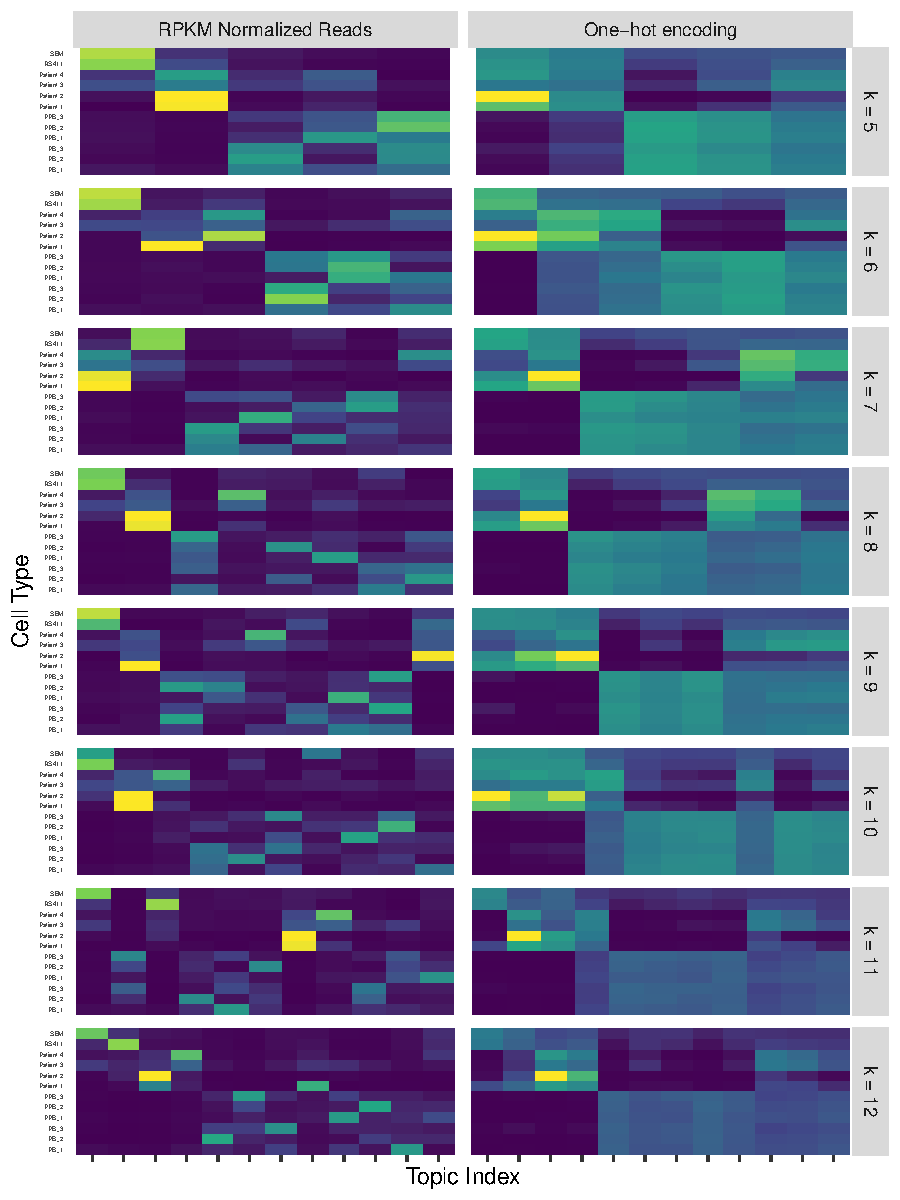
\includegraphics[width=\textwidth]{plot/ch5/mll_redo_topic_mtx.pdf}
    \caption{Inferred topic loadings for $k = 5, \ldots, 12$ topics comparing MLL-AF4 cells to B cell precursors. RPKM normalised refers to the count matrix used to infer the topic loadings by BLDA, while one-hot encoding simply annotates which regions are called as peaks by LanceOTron. Topic loadings are normalised such that the sum of all topics within a cell equals one.}
    \label{fig:mll_all_topic}
\end{figure}

Higher values of $k$ appear to impose too much structure on the data. This is evident for the BLDA case, which identifies one topic enriched for each cell type (except patient 2) at $k=12$. The OHE case interestingly deals with the over-parameterization problem differently, prefering to retain the structure seen in lower values of $k$ but assign many different topics with very low loadings within these groups. Though neither of these results are unexpected, the level of granularity for BLDA and non-specificity for OHE make it difficult to study the co-accessible regulatory elements shared between similar cell types. For that reason, we primarily are interested in the analyses for smaller values of $k$.

We select the simplest model for further analysis. We base our decision on the extremely specific topic loadings identified in the BLDA case (a single topic representing the cell lines, another involved in patients, with some sharing between them) as well as the common structure identified in PB cells separate from PPB cells with a single topic explaining the shared accessibility profile between them both. We repeat the analysis ten times for both BLDA and OHE. 

\begin{figure}
    \centering
    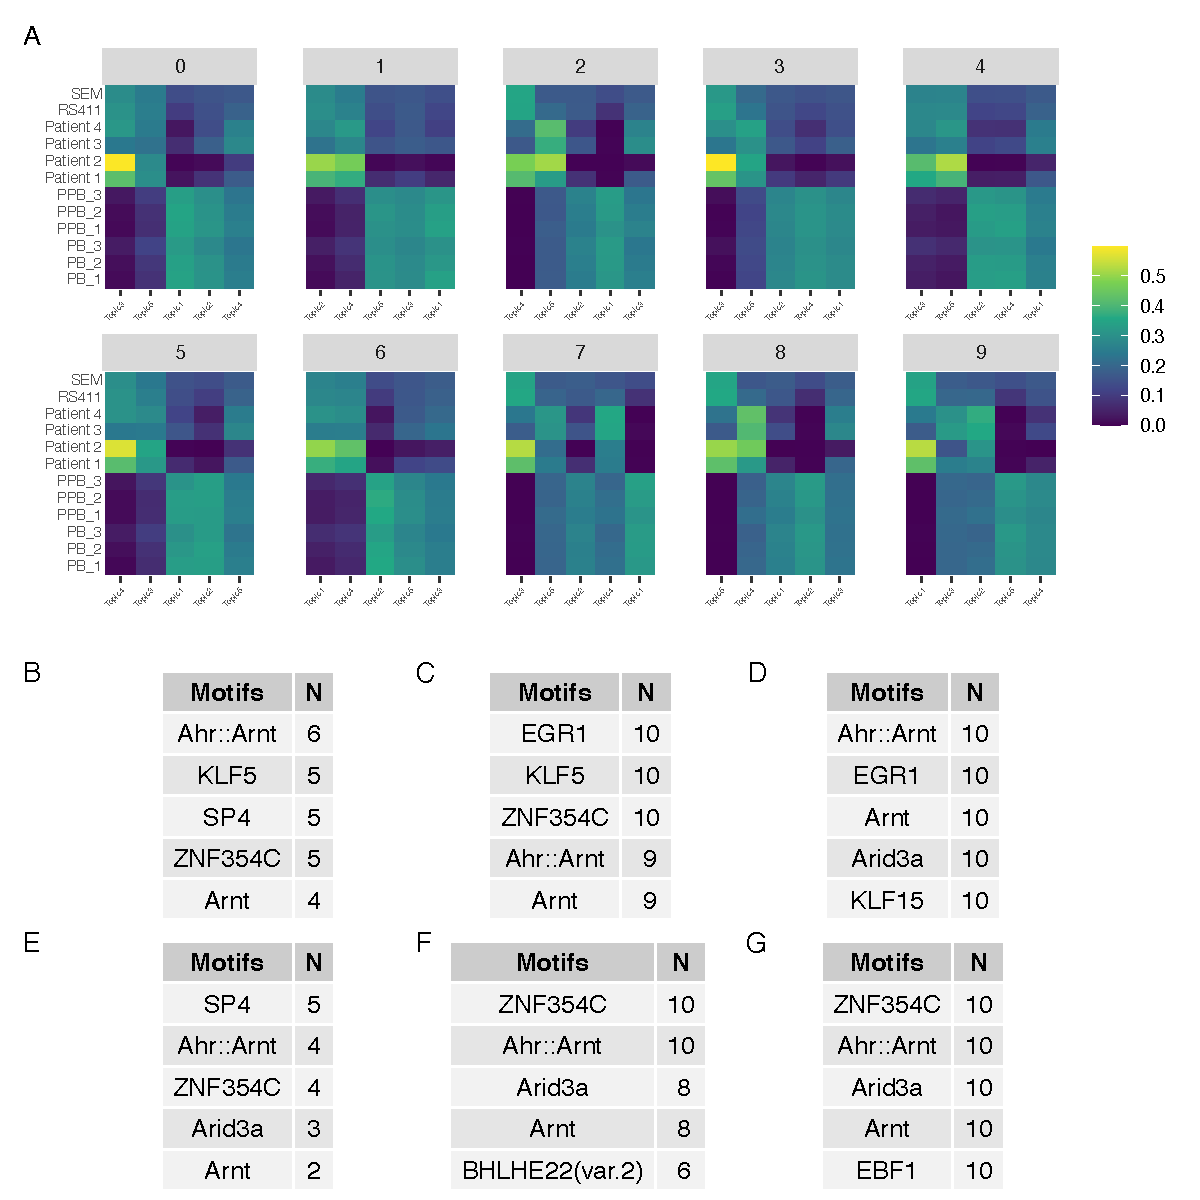
\includegraphics[width=\textwidth]{plot/ch5/mll_redo_dummy_reps.pdf}
    \caption{Ten replicates of topic modelling using one-hot encoded input. A. Inferred topic loadings on each of the samples for all 10 replicates, sorted by median topic activation. B, C, and D show the top 5 motifs identified in $N$ of the replicates in the top 100, 250, and 500 regions of manually annotated MLL-AF4 specific topics. E, F, and G show an equivalent for BCP specific topics.}
    \label{fig:mll_redo_topics}
\end{figure}

The $k=5$ OHE analysis consistently identifies at least one topic which is active in all of the MLL-AF4 cells and none of the \gls{bcp} samples (\Cref{fig:mll_redo_topics}). Patient 2 is usually the most active representative of this group within that topic. Some replicates (i.e. replicates 2, 5, 6, 7, 8, 9) also find topics active in all of the \gls{bcp} and few of the MLL-AF4 samples. There is no obvious substructure within the \gls{bcp} samples.  We manually annotate each topic as "enriched in MLL-AF4 cells", "enriched in \gls{bcp}", or neither and perform enrichment for each of the two specific sets relative to the other topics.  Motifs found in the MLL-AF4 speciifc topics in the top 100, 250, and 500 regions include SP4, KLF5, EGR1, and KLF15 (\Cref{fig:mll_redo_topics}B, C, D). Ahr::Arnt, ZNF354C, Arid3a, and Arnt are identified but found broadly between MLL-AF4 and \gls{bcp} regions.  The latter were additionally enriched for BHLHE22 and EBF1 which is a marker for B cell lineage commitment \cite{Infante2013} along with PAX5 which is occasionally identified in \gls{bcp} specific regions (data not shown). The list of motifs presented is reasonably unspecific, though there is evidence that EGR1 has deep functional relationships with many hematological malignancies including \gls{all} \cite{Tian2016}. The fact that there is at least one known system specific transcription factor whose motif is enriched for each set of samples is reassuring.  It is additionally reassuring that these important motifs were identified in each of the ten replicates in their respective sets.  Even in this low-resolution OHE setup, the technique has some power to robustly identify relevant biology across replicates.

\begin{figure}
    \centering
    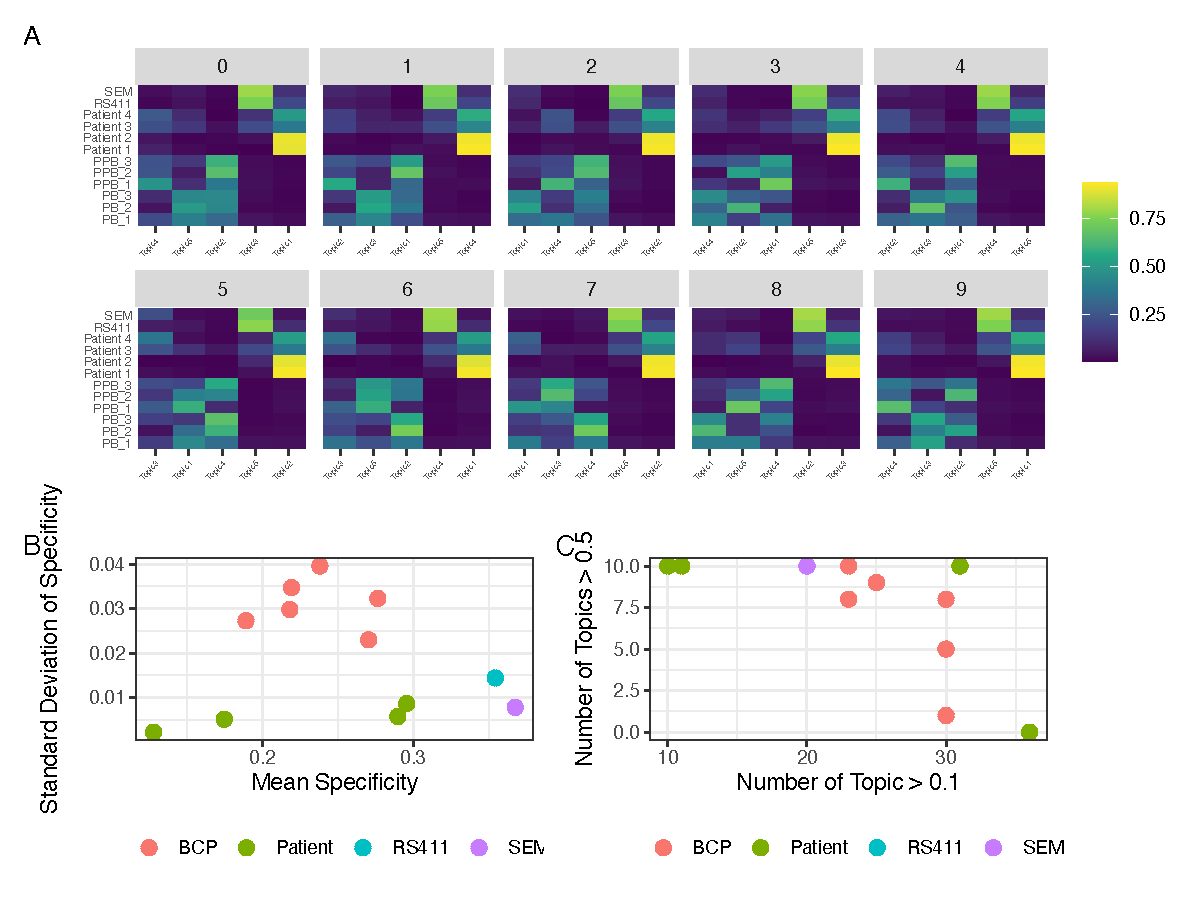
\includegraphics[width=\textwidth]{plot/ch5/mll_redo_reps_bigwig.pdf}
    \caption{Ten replicates of topic modelling using RPKM normalized input, aka BLDA. A. Inferred topic loadings for each of the 12 samples and all 10 replicates, sorted by standard deviation of topic loading. B. Mean versus standard deviation of specificity, here defined as the contribution of the most enriched topic to that sample divided by the sum of that topics enrichment to all other samples. Averaged over replicate. C. The number of instances where a sample has a topic identified above a loading value of 0.1 versus the number of instances where any topic is annotated above 0.5. Values represent contribution of a particular topic to a particular cell, such that the sum of topic loadings within a particular cell equals 1.}
    \label{fig:mll_reps}
\end{figure}

The inferred topic loadings in the BLDA case are also reproducible across replicates (\Cref{fig:mll_reps}A). In each of the 10 replicates, one topic loads preferentially onto Patients 1 and 2, and to a lesser degree onto patients 3 and 4. Another loads preferentially onto RS411 and SEM. The remainder are somewhat divided between a common co-accessibility program amongst all samples (i.e. topic 3 in replicate 5), specifically loading onto PPB (i.e. topic 5 in replicate 6), or PB (Topic 5 in replicate 0). In general, each of the replicates has at least one topic that falls into each of these categories, though the loadings onto the \gls{bcp} are less consistent than the MLL-AF4 cells. The topics loading onto RS411 and SEM were highly specific to those two samples, in contrast to the BCPs whose specificity was much lower, and additionally much more variable (\Cref{fig:mll_reps}B).  The BCPs additionally had many topics annotated to them at low levels, but very few with a higher annotation level of 0.5 (\Cref{fig:mll_reps}C).  This is in contrast to Patients 1 and 2, who had both a large number of highly specific topics across the replicates, and also a very low number of non-specific topics.  From this we conclude that similar topics are able to be found consistently across replicates.  

Having established a high degree of specificity for individual topics to the expected annotations of the samples, we investigate the regions making up the topics. We briefly focus on a single replicate, indexed as 0 in \Cref{fig:mll_reps}. An interesting avenue for exploration is the degree to which the topics are made up of similar regions. If they were, it would represent a shared core of co-accessible elements. The alternative, of completely separate underlying regions, is equally interesting. An understanding of the region-topic distribution over cell types will aid in the interpretation of the key regions for particular topics. We transform each region-topic vector to $Z$-scores by subtracting the mean and dividing by the standard deviation of the distribution, and count the number of regions with a $Z$-score over 3 (98.8 percent of a theoretical standard normal distribution) in each of the topics (\Cref{fig:mll_region_sharing}). 

\begin{figure}
    \centering
    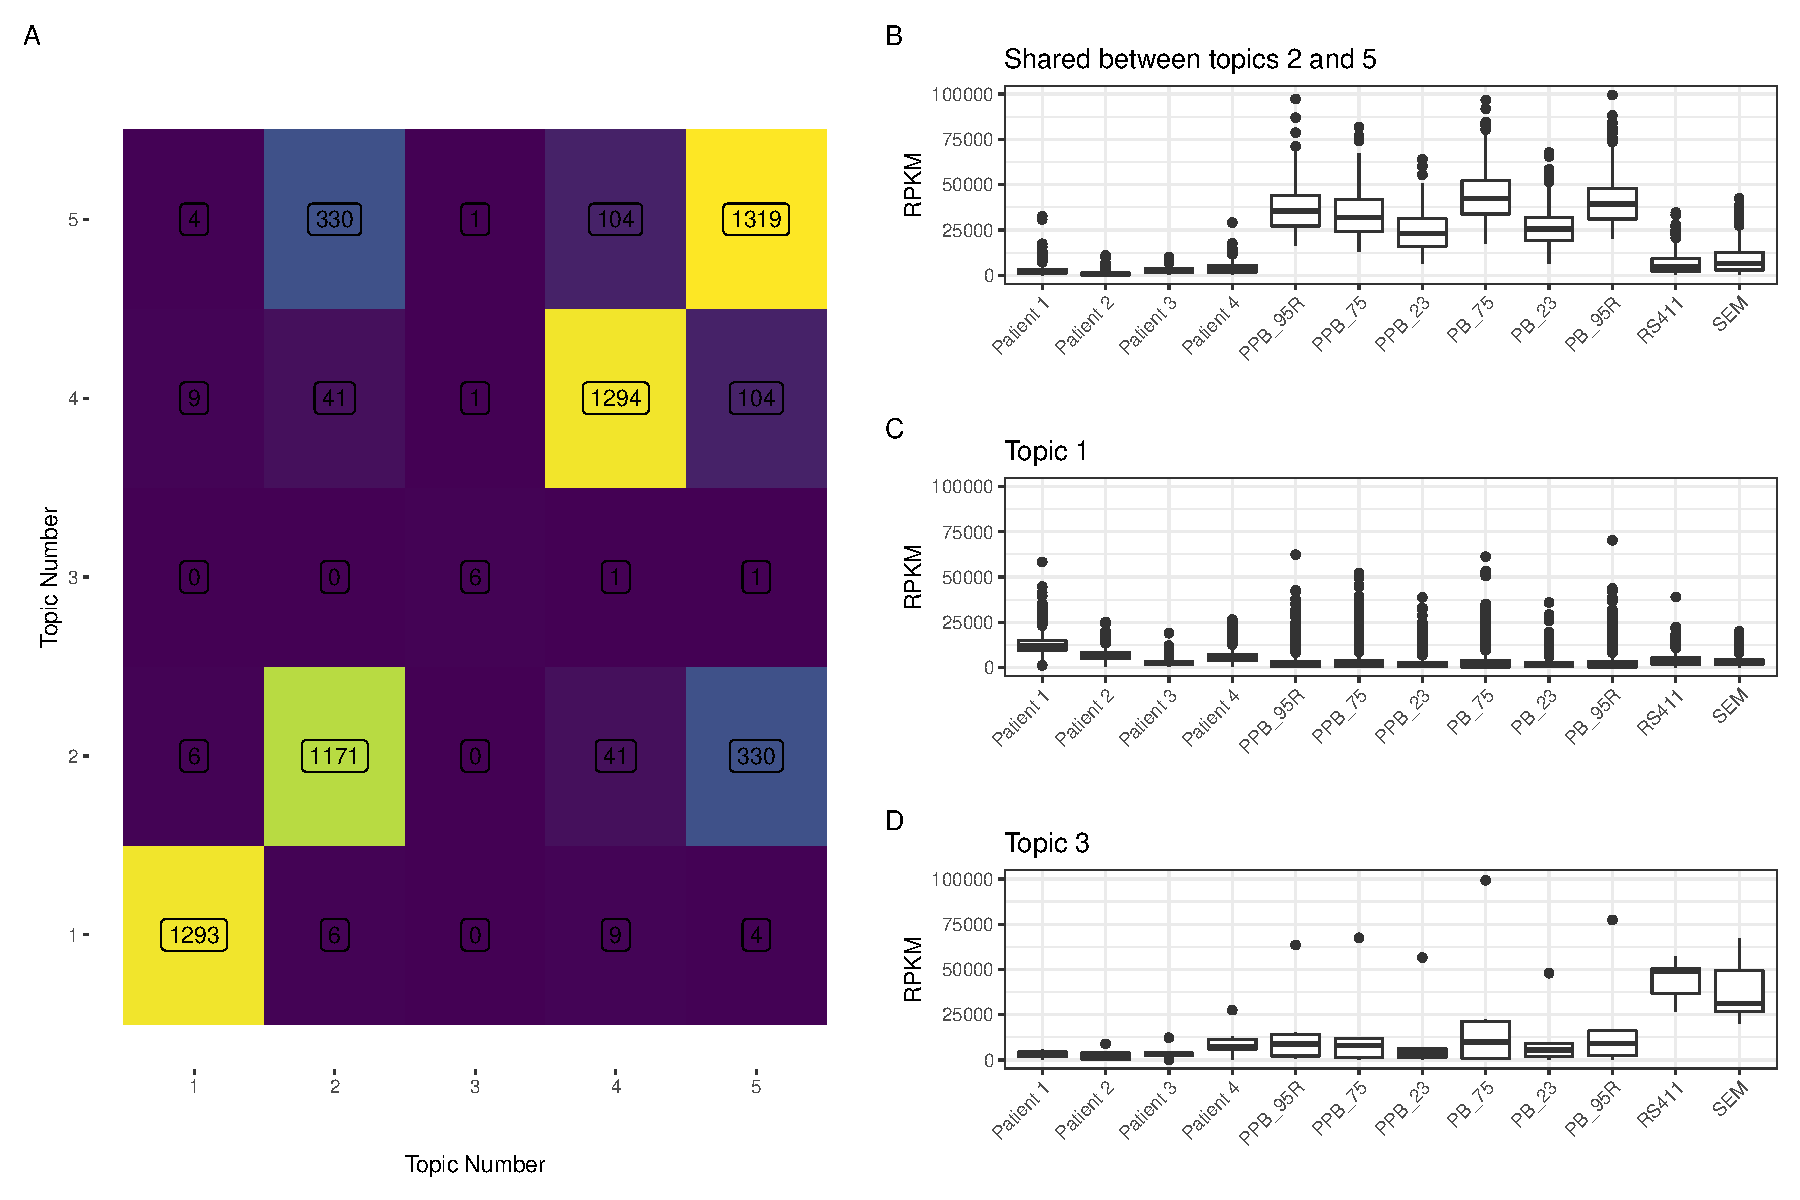
\includegraphics[width=\textwidth]{plot/ch5/mll_bigwig_region_sharing_plot_rep0.pdf}
    \caption{Regions highly annotated on each of the five topics in replicate 0 for the BLDA topic modelling. A. Region-topic loadings were converted to Z scores by subtracting the mean of the distribution and dividing by the standard deviation. Regions with a $Z$ score of 3 or more were selected, and the number of shared highly loaded regions is plotted. The number identified per topic is plotted on the diagonal. B. RPKM values for the 330 regions highly loaded for both topics 2 and 5. In this replicate, these topics were enriched in BCPs. C. RPKM values for regions highly loaded with topic 1, which primarily loads onto patient samples. D. RPKM values for the 6 regions highly loaded with topic 3, which is enriched in RS411 and SEM samples.}
    \label{fig:mll_region_sharing}
\end{figure}



%\begin{figure}
%    \centering
%    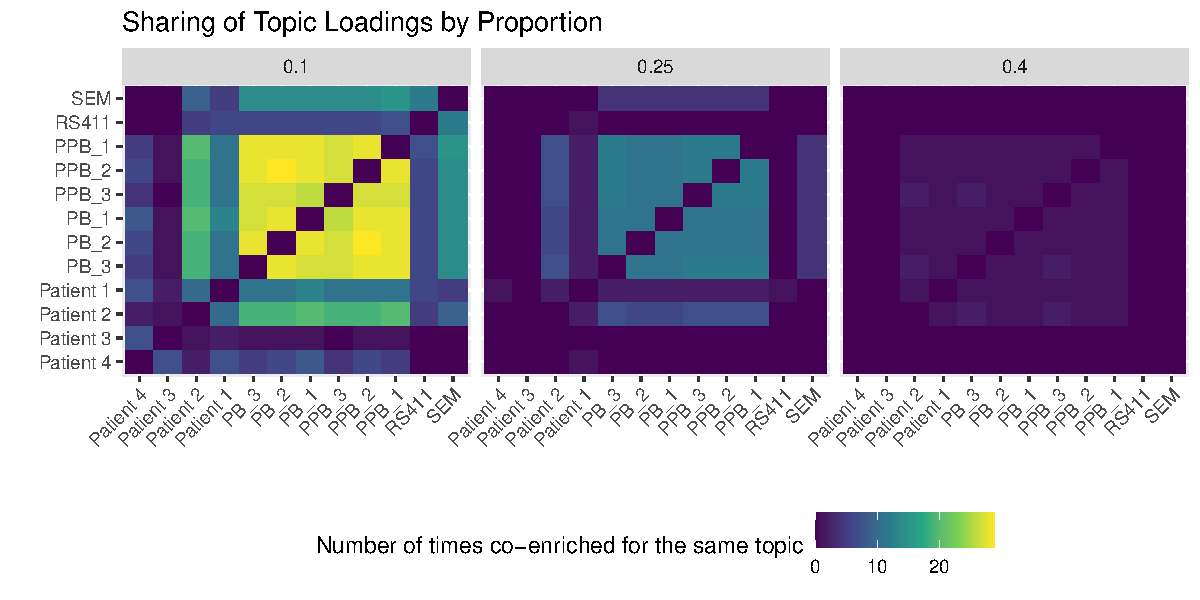
\includegraphics[width=\textwidth]{plot/ch5/mll_coenriched.pdf}
%    \caption{Degree of shared topic activity between cell types. Plotted are the number of instances where a topic is active at the facetted level in both of the indicated cell types. Results are tabulated across all $k=5, \ldots, 12$ inference runs.}
%    \label{fig:mll_shared_topics}
%\end{figure}

%Due to the high degree of topic coenrichment within the \glspl{bcp}, inference with the higher values of $k$ tends to spuriously split topic loadings. This is evident in both the OHE and BLDA cases, where the average topic loadings are very low for higher values of $k$. Additonally, RS4;11 is almost always annotated as having at least highly specific topic loading (topic 3 in $k=5, 6$, topic 4 in $k=8$). The utility of forcing a high number of topics on this system is, therefore, questionable.

%For these reasons, we initially focus our examination on the smallest number of topics (\Cref{fig:mll_k_5}). Many of the previously mentioned trends are even more evident in this small system.